\pt{\section{Funções \texorpdfstring{$(\alpha, \lambda)$}{(alpha, lambda)}-limitadas}}
\en{\section{\texorpdfstring{$(\alpha, \lambda)$}{(alpha, lambda)}-bounded functions}}
\vspace{1cm}

\pt{A definição de $(\alpha,\lambda)$-limitada é inicialmente apresentada como uma propriedade pontual, assim como a definição de continuidade:}
\en{The definition of $(\alpha,\lambda)$-bounded is initially presented as a pointwise property, just like the definition of continuity:}

\begin{definition}
  \pt{Sejam $\alpha, \lambda \ge 0$, $(X, d_X)$ e $(Y, d_Y)$ espaços métricos, $\mathcal{X} \subseteq X$. Uma função $f \colon \mathcal{X} \to Y$ é dita \textit{$(\alpha,\lambda)$-limitada no ponto $x \in \mathcal{X}$} quando, para todo $\tilde{x} \in \mathcal{X}$ tal que $d_X(x, \tilde{x}) \le \lambda$, temos $d_Y(f(x), f(\tilde{x})) \le \alpha$.}
  \en{Let $\alpha, \lambda \ge 0$, $(X, d_X)$ and $(Y, d_Y)$ be metric spaces, $\mathcal{X} \subseteq X$. A function $f \colon \mathcal{X} \to Y$ is said to be \textit{$(\alpha,\lambda)$-bounded at the point $x \in \mathcal{X}$} when, for every $\tilde{x} \in \mathcal{X}$ such that $d_X(x, \tilde{x}) \le \lambda$, we have $d_Y(f(x), f(\tilde{x})) \le \alpha$.}
\end{definition}

\begin{figure}[h!]
  \begin{center}
    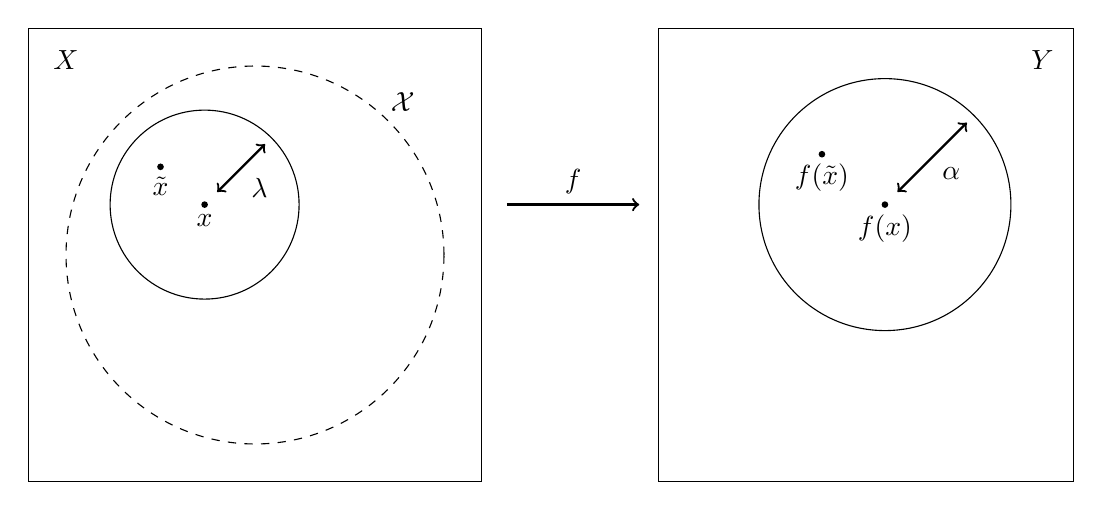
\begin{tikzpicture}[scale=.8]
      \node (X) at (-3, 3.1) {$X$};
      \node (Y) at (12.5, 3.1) {$Y$};

      \draw (-3.6, -3.6) rectangle (3.6, 3.6);
      \draw (6.4, -3.6) rectangle (13, 3.6);

      \fill (-0.8, 0.8) circle (1.5pt);
      \node[below] (x) at (-0.8, 0.8) {$x$};

      \fill (-1.5, 1.4) circle (1.5pt);
      \node[below] (xt) at (-1.5, 1.4) {$\tilde{x}$};

      \fill (10, 0.8) circle (1.5pt);
      \fill (9.0, 1.6) circle (1.5pt);
      \node[below] (y) at (10, 0.8) {$f(x)$};
      \node[below] (yt) at (9.0, 1.6) {$f(\tilde{x})$};

      \draw[dashed] (0, 0) ellipse (3cm and 3cm) node[above right, xshift=1.6cm, yshift=1.7cm] {$\mathcal{X}$};
      \draw[] (-0.8, 0.8) ellipse (1.5cm and 1.5cm);
      \draw[<->, thick] (-0.6, 1) -- ++(0.76, 0.76) node[midway, below right] {$\lambda$};
      \draw[] (10, 0.8) ellipse (2cm and 2cm);
      \draw[<->, thick] (10.2, 1) -- ++(1.1, 1.1) node[midway, below right] {$\alpha$};
      \draw[->, thick] (4, 0.8) -- (6.1, 0.8) node[midway, above] {$f$};
    \end{tikzpicture}
  \end{center}
  \captionsetup{justification=centering}
  \caption{
    \pt{Função $f : \mathcal{X} \to Y$ $(\alpha, \lambda)$-limitada em $x$.}
    \en{Function $f : \mathcal{X} \to Y$ which is $(\alpha, \lambda)$-bounded at $x$.}
  }
\end{figure}

\vspace{1cm}

\begin{definition}
  \pt{Sejam $\alpha, \lambda \ge 0$, $(X, d_X)$ e $(Y, d_Y)$ espaços métricos, $\mathcal{X} \subseteq X$. Uma função $f \colon \mathcal{X} \to Y$ é dita \textit{$(\alpha,\lambda)$-limitada} quando, para todo $x$ em $\mathcal{X}$, $f$ é $(\alpha,\lambda)$-limitada no ponto $x$.}
  \en{Let $\alpha, \lambda \ge 0$, $(X, d_X)$ and $(Y, d_Y)$ be metric spaces, $\mathcal{X} \subseteq X$. A function $f \colon \mathcal{X} \to Y$ is said to be \textit{$(\alpha,\lambda)$-bounded} when, for every $x$ in $\mathcal{X}$, $f$ is $(\alpha,\lambda)$-bounded at the point $x$.}
\end{definition}

\pt{Note que, para $\lambda = 1$, a definição acima adapta naturalmente a condição de Hölder para a ordem $0$ e coeficiente $\alpha$ (veja \cite{holder}). Também é importante notar que muitos resultados de funções contínuas não se estendem para funções $(\alpha, \lambda)$-limitadas. Veja o exemplo abaixo.}
\en{Note that, for $\lambda = 1$, the above definition naturally adapts Hölder's condition for order $0$ and coefficient $\alpha$ (see \cite{holder}). It is also important to note that many results for continuous functions do not extend to $(\alpha, \lambda)$-bounded functions. See the example below.}

\begin{example} \label{vitali}
  \pt{Considere $V$ um conjunto de Vitali. A função $f \colon [0, 1] \to \mathbb{R}$, definida por $f(x) = 1_V$ se $x \in (0, 1)$ e $f(x) = 1 - x$ caso contrário, é $1$-limitada (considerando a métrica usual) mas não é contínua, não possui pontos fixos e não é Lebesgue integrável (veja \cite{vitali}).}
  \en{Consider $V$ a Vitali set. The function $f \colon [0, 1] \to \mathbb{R}$, defined by $f(x) = 1_V$ if $x \in (0, 1)$ and $f(x) = 1 - x$ otherwise, is $1$-bounded (considering the usual metric) but is not continuous, has no fixed points, and is not Lebesgue integrable (see \cite{vitali}).}
\end{example}

\pt{Ao alterar a métrica, podemos considerar $\lambda = 1$ na definição acima sem perda de generalidade, porque $(X, d_X)$ é um espaço métrico se, e somente se, $(X, \lambda d_X)$ é um espaço métrico para todo $\lambda > 0$. Se desejarmos ter $d_X(x, \tilde{x}) \le \lambda$ para algum $\lambda > 0$, então podemos considerar o espaço métrico $(X, \frac{1}{\lambda} d_X)$ ao invés de $(X, d_X)$. Como nosso principal interesse neste trabalho são as funções $(k,1)$-limitadas, diremos que uma função é $\alpha$-limitada quando for $(\alpha,1)$-limitada.}
\en{By changing the metric, we can consider $\lambda = 1$ in the above definition without loss of generality, because $(X, d_X)$ is a metric space if and only if $(X, \lambda d_X)$ is a metric space for every $\lambda > 0$. If we wish to have $d_X(x, \tilde{x}) \le \lambda$ for some $\lambda > 0$, then we can consider the metric space $(X, \frac{1}{\lambda} d_X)$ instead of $(X, d_X)$. Since our main interest in this work is in $(k,1)$-bounded functions, we will say that a function is $\alpha$-bounded when it is $(\alpha,1)$-bounded.}

\pt{Toda função $f \colon X \to \mathbb{R}$ definida em um subconjunto discreto de $\mathbb{R}$ é contínua considerando a métrica induzida por $\mathbb{R}$, mas pode não ser $\alpha$-limitada para qualquer $\alpha > 0$. Veja a seguir.}
\en{Every function $f \colon X \to \mathbb{R}$ defined on a discrete subset of $\mathbb{R}$ is continuous considering the metric induced by $\mathbb{R}$, but it may not be $\alpha$-bounded for any $\alpha > 0$. See below.}

\begin{example} \label{two_to_n}
  \pt{$f \colon \mathbb{Z} \to \mathbb{Z}$ dada por $n \mapsto 2^n$ não é $\alpha$-limitada (considerando a métrica usual) para nenhum $\alpha > 0$, pois $f(n + 1) - f(n) = 2^{n}$ é ilimitada. Pela mesma razão, $g\colon \mathbb{Z} \to \mathbb{Z}$ dada por $n \mapsto n^2$ não é $\alpha$-limitada para nenhum $\alpha > 0$.}
  \en{$f \colon \mathbb{Z} \to \mathbb{Z}$ given by $n \mapsto 2^n$ is not $\alpha$-bounded (considering the usual metric) for any $\alpha > 0$, since $f(n + 1) - f(n) = 2^{n}$ is unbounded. For the same reason, $g\colon \mathbb{Z} \to \mathbb{Z}$ given by $n \mapsto n^2$ is not $\alpha$-bounded for any $\alpha > 0$.}
\end{example}

\pt{Abaixo estão alguns resultados imediatos da definição de função $\alpha$-limitada.}
\en{Below are some immediate results from the definition of $\alpha$-bounded function.}

\begin{theorem}
  \pt{Toda função $\alpha$-limitada é $(\alpha+\epsilon)$-limitada para todo $\epsilon > 0$.}
  \en{Every $\alpha$-bounded function is $(\alpha+\epsilon)$-bounded for every $\epsilon > 0$.}
\end{theorem}
\begin{proof}
  \pt{Evidente.}
  \en{Immediate.}
\end{proof}

\pt{Apresentamos agora a seguinte definição bem conhecida, para então relacioná-la com as funções $\alpha$-limitadas.}
\en{We now present the following well-known definition, to then relate it to $\alpha$-bounded functions.}

\begin{definition*}
  \pt{Sejam $(X, d_X)$ e $(Y, d_Y)$ espaços métricos. Uma função $f \colon X \to Y$ é dita \textit{Lipschitz contínua} se existe uma constante real $K \ge 0$ tal que para quaiser $x_1, x_2 \in X$ vale que \[d_Y\left(f(x_1), f(x_2)\right) \le K d_X\left(x_1, x_2\right).\]}
  \en{Let $(X, d_X)$ and $(Y, d_Y)$ be metric spaces. A function $f \colon X \to Y$ is said to be \textit{Lipschitz continuous} if there exists a real constant $K \ge 0$ such that for any $x_1, x_2 \in X$ it holds that \[d_Y\left(f(x_1), f(x_2)\right) \le K d_X\left(x_1, x_2\right).\]}
\end{definition*}

\begin{theorem}
  \pt{Sejam $(X, d_X)$ e $(Y, d_Y)$ espaços métricos, $\mathcal{X} \subseteq X$. Toda função Lipschitz contínua, com constante $K$, $f \colon \mathcal{X} \to Y$ é $K$-limitada.}
  \en{Let $(X, d_X)$ and $(Y, d_Y)$ be metric spaces, $\mathcal{X} \subseteq X$. Every Lipschitz continuous function, with constant $K$, $f \colon \mathcal{X} \to Y$ is $K$-bounded.}
\end{theorem}
\begin{proof}
  \pt{Para todo $x_1, x_2 \in \mathcal{X}, d_X(x_1, x_2) \le 1$ e consequentemente $d_Y(f(x_1), f(x_2)) \le K d_X(x_1, x_2) \le K$.}
  \en{For every $x_1, x_2 \in \mathcal{X}, d_X(x_1, x_2) \le 1$ and consequently $d_Y(f(x_1), f(x_2)) \le K d_X(x_1, x_2) \le K$.}
\end{proof}

\pt{Note que nem todas as funções $\alpha$-Hölder contínuas são $\beta$-limitadas para algum $\beta > 0$. A função $\sqrt{\cdot} \colon \mathbb{R}^+ \to \mathbb{R}$ constitui um contraexemplo (considerando a métrica usual) pelo mesmo motivo mencionado no exemplo \ref{two_to_n}.}
\en{Note that not all $\alpha$-Hölder continuous functions are $\beta$-bounded for some $\beta > 0$. The function $\sqrt{\cdot} \colon \mathbb{R}^+ \to \mathbb{R}$ constitutes a counterexample (considering the usual metric) for the same reason mentioned in example \ref{two_to_n}.}

\begin{theorem}
  \pt{Sejam $(X, d_X)$ e $(Y, d_Y)$ espaços métricos, $\mathcal{X} \subseteq X$, e $f \colon \mathcal{X} \to Y$ uma função. Se para todo $\epsilon > 0$ existe um $\alpha \in (0, \epsilon]$ tal que $f$ é $\alpha$-limitada, então $f$ é contínua.}
  \en{Let $(X, d_X)$ and $(Y, d_Y)$ be metric spaces, $\mathcal{X} \subseteq X$, and $f \colon \mathcal{X} \to Y$ a function. If for every $\epsilon > 0$ there exists an $\alpha \in (0, \epsilon]$ such that $f$ is $\alpha$-bounded, then $f$ is continuous.}
\end{theorem}
\begin{proof}
  \pt{Com efeito, para cada $x \in \mathcal{X}, \epsilon > 0$, existe algum $\alpha \in (0, \epsilon]$ tal que $\tilde{x} \in \mathcal{X}, d_X(x, \tilde{x}) \le 1 \implies d_Y(f(x), f(\tilde{x})) \le \alpha \le \epsilon$.}
  \en{Indeed, for each $x \in \mathcal{X}, \epsilon > 0$, there is some $\alpha \in (0, \epsilon]$ such that $\tilde{x} \in \mathcal{X}, d_X(x, \tilde{x}) \le 1 \implies d_Y(f(x), f(\tilde{x})) \le \alpha \le \epsilon$.}
\end{proof}

\begin{theorem}
  \pt{Sejam $(X, d_X)$ e $(Y, d_Y)$ espaços métricos, $\mathcal{X} \subseteq X$. Se $(f_n) \to f$ ponto a ponto, $f_n \colon \mathcal{X} \to Y$ são $\alpha$-limitadas para todo $n \in \mathbb{Z}_{> 0}$, então $f$ é $\alpha$-limitada.}
  \en{Let $(X, d_X)$ and $(Y, d_Y)$ be metric spaces, $\mathcal{X} \subseteq X$. If $(f_n) \to f$ pointwise, $f_n \colon \mathcal{X} \to Y$ are $\alpha$-bounded for every $n \in \mathbb{Z}_{> 0}$, then $f$ is $\alpha$-bounded.}
\end{theorem}
\begin{proof}
  \pt{Suponha, por contradição, que $f$ não seja $\alpha$-limitada. Então existem $x_1, x_2 \in \mathcal{X}$, $d_X(x_1, x_2) \le 1$, tal que $d_Y(f(x_1), f(x_2)) \coloneqq k > \alpha$. Como $(f_n) \to f$ ponto a ponto, existe algum $n \in \mathbb{Z}_{> 0}$ com $d_Y(f_n(x_1), f(x_1)) < \frac{k - \alpha}{2}$ e $d_Y(f_n(x_2), f(x_2)) < \frac{k - \alpha}{2}$. Consequentemente, $d_Y(f_n(x_1), f_n(x_2)) > k - \frac{k - \alpha}{2} - \frac{k - \alpha}{2} = \alpha$, uma contradição.}
  \en{Suppose, for a contradiction, that $f$ is not $\alpha$-bounded. Then there are $x_1, x_2 in \mathcal{X}$, $d_X(x_1, x_2) \le 1$, such that $d_Y(f(x_1), f(x_2)) \coloneqq k > \alpha$. As $(f_n) \to f$ pointwise, there is some $n in \mathbb{Z}_{> 0}$ with $d_Y(f_n(x_1), f(x_1)) < \frac{k - \alpha}{2}$ and $d_Y(f_n(x_2), f(x_2)) < \frac{k - \alpha}{2}$. Consequently, $d_Y(f_n(x_1), f_n(x_2)) > k - \frac{k - \alpha}{2} - \frac{k - \alpha}{2} = \alpha$, a contradiction.}
\end{proof}

\pt{As funções $\alpha$-limitadas podem não ser o limite pontual de qualquer sequência de funções contínuas.}
\en{The $\alpha$-bounded functions may not be the pointwise limit of any sequence of continuous functions.}

\begin{example}
  \pt{A função de Dirichlet $1_\mathbb{Q} \colon [0, 1] \to \mathbb{R}$, também conhecida como função indicadora dos racionais, é $1$-limitada considerando a métrica usual de $\mathbb{R} \supset [0, 1]$, mas não é o limite pontual de nenhuma sequência de funções contínuas, pois é uma função da classe 2 de Baire (veja \cite{baire}).}
  \en{The Dirichlet function $1_\mathbb{Q} \colon [0, 1] \to \mathbb{R}$, also known as the indicator function of the rationals, is $1$-bounded considering the usual metric of $\mathbb{R} \supset [0, 1]$, but it is not the pointwise limit of any sequence of continuous functions, as it is a class 2 Baire function (see \cite{baire}).}
\end{example}

\pt{A aritmética com funções $\alpha$-limitadas não é a mesma que com funções contínuas definidas em $\mathbb{R}$.}
\en{Arithmetic with $\alpha$-bounded functions is not the same as with continuous functions defined on $\mathbb{R}$.}

\begin{theorem}
  \pt{Sejam $(X, d_X)$ e $(Y, d_Y)$ espaços métricos e $(Y, +_Y, \cdot_Y)$ um espaço vetorial sobre $\mathbb{R}$. Se $f \colon X \to Y$ e $g \colon X \to Y$ são duas funções $\alpha$-limitadas, então $f + g$ é $(2\alpha)$-limitada e $\gamma f$ é $(\gamma \alpha)$-limitada para todo $\gamma > 0$.}
  \en{Let $(X, d_X)$ and $(Y, d_Y)$ be metric spaces and $(Y, +_Y, \cdot_Y)$ a vector space over $\mathbb{R}$. If $f \colon X \to Y$ and $g \colon X \to Y$ are two $\alpha$-bounded functions, then $f + g$ is $(2\alpha)$-bounded and $\gamma f$ is $(\gamma \alpha)$-bounded for every $\gamma > 0$.}
\end{theorem}

\begin{proof}
  \pt{Se $x \in X$ e $\tilde{x} \in X$, $d_X(x, \tilde{x}) \le 1$, então $f(\tilde{x}) \in \overline{B}_{\alpha}(f(x))$ e $g(\tilde{x}) \in \overline{B}_{\alpha}(g(x))$, portanto $(f + g)(\tilde{x}) = f(\tilde{x}) + g(\tilde{x}) \in \overline{B}_{2\alpha}((f + g)(x))$, e consequentemente $f + g$ é $(2\alpha)$-limitada. Analogamente, $(\gamma f)(\tilde{x}) \in \overline{B}_{\gamma \alpha}(f(x))$ e $\gamma f$ é $(\gamma \alpha)$-limitada.}
    \en{If $x \in X$ and $\tilde{x} \in X$, $d_X(x, \tilde{x}) \le 1$, then $f(\tilde{x}) \in \overline{B}_{\alpha}(f(x))$ and $g(\tilde{x}) \in \overline{B}_{\alpha}(g(x))$, therefore $(f + g)(\tilde{x}) = f(\tilde{x}) + g(\tilde{x}) \in \overline{B}_{2\alpha}((f + g)(x))$, and consequently $f + g$ is $(2\alpha)$-bounded. Similarly, $(\gamma f)(\tilde{x}) \in \overline{B}_{\gamma \alpha}(f(x))$ and $\gamma f$ is $(\gamma \alpha)$-bounded.}
\end{proof}

\pt{O teorema acima permite considerar espaços vetoriais de mapas entre dois espaços métricos que são $\alpha$-limitados para algum $\alpha \ge 0$.}
\en{The above theorem allows considering vector spaces of maps between two metric spaces that are $\alpha$-bounded for some $\alpha \ge 0$.}

\pt{O produto de duas funções $\alpha$-limitadas (com o mesmo domínio e contradomínio) pode não ser $\beta$-limitado para nenhum $\beta > 0$, assim como o recíproco de uma função $\alpha$-limitada (quando definido).}
\en{The product of two $\alpha$-bounded functions (with the same domain and codomain) may not be $\beta$-bounded for any $\beta > 0$, as well as the reciprocal of an $\alpha$-bounded function (when defined).}

\begin{example}
  \pt{$f \colon \mathbb{Z}_{> 0} \to \mathbb{Z}_{> 0}$ dada por $f(n) = n$ é $1$-limitada (considerando a métrica usual), mas $f^2$ coincide com $g \colon \mathbb{R} \to \mathbb{R}$, $g(x) = x^2$, portanto não é $\alpha$-limitada para nenhum $\alpha > 0$.}
  \en{$f \colon \mathbb{Z}_{> 0} \to \mathbb{Z}_{> 0}$ given by $f(n) = n$ is $1$-bounded (considering the usual metric), but $f^2$ coincides with $g \colon \mathbb{R} \to \mathbb{R}$, $g(x) = x^2$, therefore it is not $\alpha$-bounded for any $\alpha > 0$.}
\end{example}

\begin{example}
  \pt{$f \colon [1, +\infty) \to \mathbb{R}$ dada por $f(x) = \frac{1}{x^2}$ é $1$-limitada, mas $\frac{1}{f}$ coincide com $g \colon \mathbb{R} \to \mathbb{R}$, $g(x) = x^2$, portanto não é $\alpha$-limitada para nenhum $\alpha > 0$.}
  \en{$f \colon [1, +\infty) \to \mathbb{R}$ given by $f(x) = \frac{1}{x^2}$ is $1$-bounded, but $\frac{1}{f}$ coincides with $g \colon \mathbb{R} \to \mathbb{R}$, $g(x) = x^2$, therefore it is not $\alpha$-bounded for any $\alpha > 0$.}
\end{example}

\pt{O teorema de extensão para funções $\alpha$-limitadas não é muito forte.}
\en{The extension theorem for $\alpha$-bounded functions is not very strong.}

\begin{theorem} \label{tietze}
  \pt{Sejam $(X,d_X)$ e $(Y, d_Y)$ espaços métricos, $\mathcal{X}, \tilde{\mathcal{X}} \subset X$, onde $\tilde{\mathcal{X}}$ é finito, e seja $f \colon \mathcal{X} \to Y$ uma função $(\alpha,\lambda)$-limitada. Existe $\beta \ge 0$ tal que $f$ tem uma extensão $(\beta,\lambda)$-limitada para $\mathcal{X} \cup \tilde{\mathcal{X}}$ se e somente se $f$ é limitada em $\overline{B}_{\lambda}(\tilde{x}) \cap \mathcal{X}$ para cada $\tilde{x} \in \tilde{\mathcal{X}}$.}
  \en{Let $(X,d_X)$ and $(Y, d_Y)$ be metric spaces, $\mathcal{X}, \tilde{\mathcal{X}} \subset X$, where $\tilde{\mathcal{X}}$ is finite, and let $f \colon \mathcal{X} \to Y$ be an $(\alpha,\lambda)$-bounded function. There exists $\beta \ge 0$ such that $f$ admits a $(\beta,\lambda)$-bounded extension to $\mathcal{X} \cup \tilde{\mathcal{X}}$ if and only if $f$ is bounded on $\overline{B}_{\lambda}(\tilde{x}) \cap \mathcal{X}$ for each $\tilde{x} \in \tilde{\mathcal{X}}$.}
\end{theorem}

\begin{proof}
  \pt{A necessidade dessa condição é evidente. Vamos então provar que ela é suficiente.

    Podemos supor que $\tilde{\mathcal{X}} \cap \mathcal{X} = \varnothing$, já que obviamente $f$ é limitada em $\overline{B}_{\lambda}(x)$ para cada $x \in \mathcal{X}$.

    Procederemos por indução sobre o número $n$ de elementos em $\tilde{\mathcal{X}}$.

    Para $n = 0$, o resultado é óbvio. Suponha que o resultado seja verdade para $n$, e $\tilde{\mathcal{X}}$ tenha $n+1$ elementos.

    Fixe $\tilde{x} \in \tilde{\mathcal{X}}$ e $y \in Y$. Por hipótese, $f$ tem uma extensão $(\beta,\lambda)$-limitada para $\mathcal{X} \cup (\tilde{\mathcal{X}} \setminus {\tilde{x}})$. Defina $\tilde{f} \colon \mathcal{X} \cup \tilde{\mathcal{X}}$ por $\tilde{f}(\tilde{x}) = y$ e $\tilde{f}(x) = f(x)$ para cada $x \in \mathcal{X} \cup (\tilde{\mathcal{X}} \setminus {\tilde{x}})$. Claramente existe $\gamma \ge 0$ tal que $\tilde{f}$ é $(\gamma,\lambda)$-limitada em $x$ para cada $x$ diferente de $\tilde{x}$. Mas como $f$ é limitada em $\overline{B}_{\lambda}(\tilde{x}) \cap \mathcal{X}$, existe $M \ge 0$ tal que $\lvert f(x) \rvert \le M$ para cada $x \in \overline{B}_{\lambda}(\tilde{x}) \cap \mathcal{X}$. Portanto, $\lvert \tilde{f}(x)-\tilde{f}(\tilde{x})\rvert \le \lvert f(x)\rvert + \lvert -y\rvert \le M + \lvert-y\rvert$ para cada $x \in \overline{B}_{\lambda}(\tilde{x}) \cap \mathcal{X}$, e consequentemente, $\tilde{f}$ é $(\max\{M + \lvert-y\rvert, \gamma\},\lambda)$-limitada. Assim, o resultado também segue para $n+1$.}
  \en{The necessity of this condition is evident. We will now prove that it is sufficient.

    We can assume that $\tilde{\mathcal{X}} \cap \mathcal{X} = \varnothing$, since obviously $f$ is bounded on $\overline{B}_{\lambda}(x)$ for each $x \in \mathcal{X}$.

    We proceed by induction on the number $n$ of elements in $\tilde{\mathcal{X}}$.

    For $n = 0$, the result is obvious. Suppose the result holds for $n$, and $\tilde{\mathcal{X}}$ has $n+1$ elements.

    Fix $\tilde{x} \in \tilde{\mathcal{X}}$ and $y \in Y$. By hypothesis, $f$ admits a $(\beta,\lambda)$-bounded extension to $\mathcal{X} \cup (\tilde{\mathcal{X}} \setminus {\tilde{x}})$. Define $\tilde{f} \colon \mathcal{X} \cup \tilde{\mathcal{X}}$ by $\tilde{f}(\tilde{x}) = y$ and $\tilde{f}(x) = f(x)$ for each $x \in \mathcal{X} \cup (\tilde{\mathcal{X}} \setminus {\tilde{x}})$. Clearly, there exists $\gamma \ge 0$ such that $\tilde{f}$ is $(\gamma,\lambda)$-bounded at $x$ for each $x$ different from $\tilde{x}$. But since $f$ is bounded on $\overline{B}_{\lambda}(\tilde{x}) \cap \mathcal{X}$, there exists $M \ge 0$ such that $\lvert f(x) \rvert \le M$ for each $x \in \overline{B}_{\lambda}(\tilde{x}) \cap \mathcal{X}$. Therefore, $\lvert \tilde{f}(x)-\tilde{f}(\tilde{x})\rvert \le \lvert f(x)\rvert + \lvert -y\rvert \le M + \lvert-y\rvert$ for each $x \in \overline{B}_{\lambda}(\tilde{x}) \cap \mathcal{X}$, and consequently, $\tilde{f}$ is $(\max\{M + \lvert-y\rvert, \gamma\},\lambda)$-bounded. Thus, the result also holds for $n+1$.}
\end{proof}

\pt{Os exemplos abaixo ilustram por que as condições do teorema são necessárias.}
\en{The examples below illustrate why the conditions of the theorem are necessary.}

\begin{example}
  \pt{Seja $X \coloneqq \{(x, \pm 1) \mid x \in \mathbb{Z}\} \subset \mathbb{Z}^2$. Considere $f \colon X \to \mathbb{Z}$ dada por $f(x, 1) = x$ e $f(x, -1) = 0$ para qualquer $x \in \mathbb{Z}$. Claramente, $f$ é $1$-limitada, considerando a métrica usual, mas $f$ não tem nenhuma extensão $\alpha$-limitada, para qualquer $\alpha > 0$, ao conjunto $\{(x, y) \mid x \in \mathbb{Z}, y \in \{-1,0,1\}\}$, pois $\overline{B}_1((x, 0)) \supset \{ (x, 1), (x, -1) \}$ e $\lvert f(x, 1) - f(x, -1) \rvert = \lvert x - 0 \rvert$ é ilimitada.}
  \en{Let $X \coloneqq \{(x, \pm 1) \mid x \in \mathbb{Z}\} \subset \mathbb{Z}^2$. Consider $f \colon X \to \mathbb{Z}$ defined by $f(x, 1) = x$ and $f(x, -1) = 0$ for any $x \in \mathbb{Z}$. Clearly, $f$ is $1$-bounded, considering the usual metric, but $f$ has no $\alpha$-bounded extension, for any $\alpha > 0$, to the set $\{(x, y) \mid x \in \mathbb{Z}, y \in \{-1,0,1\}\}$, because $\overline{B}_1((x, 0)) \supset \{ (x, 1), (x, -1) \}$ and $\lvert f(x, 1) - f(x, -1) \rvert = \lvert x - 0 \rvert$ is unbounded.}
\end{example}

\begin{figure}[H]
  \begin{center}
    \centering
    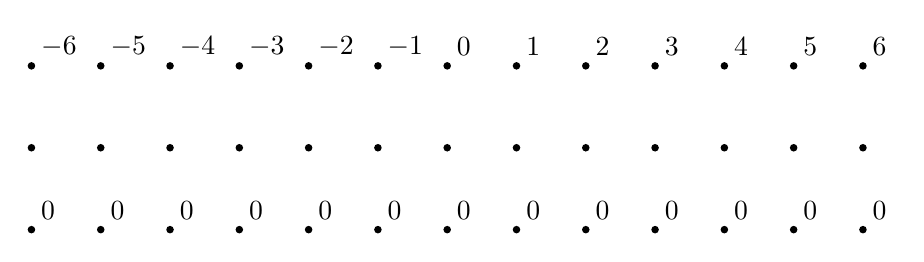
\begin{tikzpicture}[scale=0.8]
      \foreach \y in {1, 0, -1} {
          \foreach \x in {-6, ..., 6} {
              \fill[color=black] (\x*1.1+3,\y*1.3) circle (0.06);

              \ifnum\y=1
                \node[right] at (\x*1.1+3,\y*1.3+0.3) {$\x$};
              \fi
              \ifnum\y=-1
                \node[right] at (\x*1.1+3,\y*1.3+0.3) {$0$};
              \fi
            }
        }
    \end{tikzpicture}
    \captionsetup{justification=centering}
    \caption{
      \pt{Função $1$-limitada sem extensão $\alpha$-limitada, para qualquer $\alpha > 0$, para um conjunto com infinitos pontos adicionais.}
      \en{$1$-bounded function without an $\alpha$-bounded extension, for any $\alpha > 0$, for a set with infinitely many additional points.}
    }
  \end{center}
\end{figure}


\begin{example}
  \pt{Seja $s_n \in l^2(\mathbb{Z}_{> 0})$ a sequência com um $1$ na posição $n$-ésima e $0$'s nas outras posições, e $X = \{ s_n \mid n \in \mathbb{Z}_{> 0} \}$. $f \colon X \to \mathbb{Z}$ dada por $f(s_n) = n$ é $1$-limitada considerando a norma euclideana $l^2$, mas não tem nenhuma extensão $\alpha$-limitada ao conjunto $X \cup \{(0, 0, 0, \dots)\}$ para qualquer $\alpha > 0$, pois $f$ é ilimitada em $\overline{B}_1((0, 0, 0, \dots))$.}
  \en{Let $s_n \in l^2(\mathbb{Z}_{> 0})$ be the sequence with a $1$ in the $n$-th position and $0$'s in the other positions, and let $X = \{ s_n \mid n \in \mathbb{Z}_{> 0} \}$. The function $f \colon X \to \mathbb{Z}$ given by $f(s_n) = n$ is $1$-bounded considering the Euclidean $l^2$ norm, but it has no $\alpha$-bounded extension to the set $X \cup \{(0, 0, 0, \dots)\}$ for any $\alpha > 0$, since $f$ is unbounded in $\overline{B}_1((0, 0, 0, \dots))$.}
\end{example}

\begin{figure}[H]
  \begin{center}
    \begin{tikzpicture}
      \fill (0,0) circle (0.07);
      \node at ([shift={(1cm, -0.5cm)}] 0,0) {$(0, 0, \dots)$};

      % Constants
      \def\n{10} % Number of surrounding points
      \def\k{3.2}  % Constant k in the angle formula
      \def\startOffset{-77}

      % Loop to place points in a circular arrangement
      \foreach \i in {1,...,\n} {
          % Calculate angle for the point using (2 * pi / k) * log(N)
          \pgfmathsetmacro{\angle}{\startOffset + (360 / \k) * ln(\i + 1)}
          \pgfmathsetmacro{\angleout}{\startOffset + (360 / \k) * ln(\i)}


          % Coordinates of the surrounding point at radius 2
          \path (\angle:5) coordinate (P\i);
          \draw[dashed] (0, 0) -- (P\i);
          \ifnum\i>1
            \pgfmathtruncatemacro{\prev}{\i-1}
            % Calculate the start and end angles for each arc
            \pgfmathsetmacro{\startAngle}{\startOffset + (360 / \k) * ln(\prev + 1)}
            \pgfmathsetmacro{\endAngle}{\angle}
            \ifnum\i<4
              \draw[dashed]
              (P\prev) arc[start angle=\startAngle, end angle=\endAngle, radius=5]
              node[midway, above right] {\(\sqrt{2}\)}; % Label at midpoint of each edge
            \else
              \ifnum\i>4
                \draw[dashed]
                (P\prev) arc[start angle=\startAngle, end angle=\endAngle, radius=5];
              \else
                \draw[dashed]
                (P\prev) arc[start angle=\startAngle, end angle=\endAngle, radius=5]
                node[midway, above] {\(\sqrt{2}\)}; % Label at midpoint of each edge
              \fi
            \fi
          \fi


          % Draw the point and label it
          %\fill (P\i) circle (0.05) node[below left] {$s_{\i}$};

          \ifnum\i<5
            \fill[font=\bfseries] (P\i) circle (0.05) node[above left] {$s_{\i}$};
          \else
            \ifnum\i>9
              \fill (P\i) circle (0.05) node[below] {$s_{\i}$};
            \else
              \fill (P\i) circle (0.05) node[below left] {$s_{\i}$};
            \fi
          \fi
        }

      \node at ([shift={(0.5cm, -0.7cm)}] P10) {$\ddots$};

    \end{tikzpicture}
    \captionsetup{justification=centering}
    \caption{Sequência de pontos de $l^2(\mathbb{Z}_{> 0})$ na esfera unitária. A escala dos angulos que os pontos $s_n$ formam com o eixo $x$ é logarítimica em $n$.}
  \end{center}
\end{figure}


\pt{O corolário a seguir e os exemplos subsequentes ilustram algumas propriedades interessantes das funções $\alpha$-limitadas, especialmente como elas podem ser estendidas de um conjunto compacto para incluir finitos pontos adicionais.}
\en{The following corollary and subsequent examples illustrate some interesting properties of $\alpha$-bounded functions, especially how they can be extended from a compact set to include finitely many additional points.}

\begin{corollary}
  \pt{Toda função $\alpha$-limitada definida em um conjunto compacto $\mathcal{X}$ possui uma extensão $\beta$-limitada para qualquer conjunto $\tilde{\mathcal{X}} \supseteq \mathcal{X}$ tal que $\tilde{\mathcal{X}} \setminus \mathcal{X}$ é finito.}
  \en{Every $\alpha$-bounded function defined on a compact set $\mathcal{X}$ admits a $\beta$-bounded extension to any set $\tilde{\mathcal{X}} \supseteq \mathcal{X}$ such that $\tilde{\mathcal{X}} \setminus \mathcal{X}$ is finite.}
\end{corollary}
\begin{proof}
  \pt{Como $\mathcal{X}$ é compacto, a cobertura $\{ B_1(x) \mid x \in \mathcal{X} \} \supseteq \mathcal{X}$ possui uma subcobertura finita $\{ B_1(x_1), \dots, B_1(x_n)\}$.}
  \en{Since $\mathcal{X}$ is compact, the cover $\{ B_1(x) \mid x \in \mathcal{X} \} \supseteq \mathcal{X}$ has a finite subcover $\{ B_1(x_1), \dots, B_1(x_n)\}$.}

  \pt{Logo $f$ é limitada por $\max\{\lvert f(x_1) \rvert + \alpha, \dots, \lvert f(x_n) \rvert + \alpha\}$, e podemos aplicar o teorema \ref{tietze}.}
  \en{Thus, $f$ is bounded by $\max\{\lvert f(x_1) \rvert + \alpha, \dots, \lvert f(x_n) \rvert + \alpha\}$, and we can apply theorem \ref{tietze}.}
\end{proof}

\pt{Note que podemos ter $\beta < \alpha$ no teorema acima, já que $\alpha$ não precisa ser mínimo e $\tilde{\mathcal{X}} \setminus \mathcal{X}$ pode, por exemplo, ser vazio. Também não podemos assumir que $\beta = \alpha$ no teorema acima.}
\en{Note that we can have $\beta < \alpha$ in the above theorem, since $\alpha$ does not need to be minimal and $\tilde{\mathcal{X}} \setminus \mathcal{X}$ can, for example, be empty. We also cannot assume that $\beta = \alpha$ in the above theorem.}

\begin{example}
  \pt{Seja $X \coloneqq \{-1, 1\} \subset \mathbb{Z}$. A função $f \colon X \to \mathbb{Z}$ dada por $f(x) = 2x$ é $1$-limitada (considerando a métrica usual), mas não existe uma extensão $1$-limitada de $f$ para o conjunto $\{-1, 0, 1\}$ pois $\lvert f(1) - f(-1) \rvert > 1$.}
  \en{Let $X \coloneqq \{-1, 1\} \subset \mathbb{Z}$. The function $f \colon X \to \mathbb{Z}$ given by $f(x) = 2x$ is $1$-bounded (considering the usual metric), but there does not exist a $1$-bounded extension of $f$ to the set $\{-1, 0, 1\}$ since $\lvert f(1) - f(-1) \rvert > 1$.}
\end{example}

\pt{O que foi apresentado neste capítulo mostra as propriedades básicas das funções $(\alpha,\lambda)$-limitadas e como elas se comportam em comparação com funções contínuas em espaços métricos. Os teoremas e exemplos ilustram as características fundamentais dessas funções, e fornecem uma base para o estudo aprofundado das funções $(\alpha,\lambda)$-limitadas em contextos mais específicos, como o explorado no terceiro capítulo.}
\en{What has been presented in this chapter shows the basic properties of $(\alpha,\lambda)$-bounded functions and how they behave in comparison to continuous functions in metric spaces. Theorems and examples illustrate the fundamental characteristics of these functions and provide a foundation for the in-depth study of $(\alpha,\lambda)$-bounded functions in more specific contexts, such as those explored in the third chapter.}
